\documentclass[11pt,a4paper]{article}
\usepackage[utf8]{inputenc}
\usepackage{amsmath,enumitem,amsfonts,amssymb,graphicx,commath}
\usepackage{sectsty}
\usepackage{multicol}
\usepackage{tikz}

\graphicspath{ {./img/} }
\DeclareMathAlphabet{\pazocal}{OMS}{zplm}{m}{n}
\usetikzlibrary{arrows,automata}

\usepackage[%
    left=1in,%
    right=1.0in,%
    top=0.8in,%
    bottom=1in,%
]{geometry}%

\sectionfont
{\fontsize{14.4}{12}\selectfont}
\title{\textbf{Principles of AI Planning
		\\{\Large Exercise Sheet 9}}}
\makeatletter
\renewcommand{\@maketitle}
{
	\newpage
	\null
	\vskip 2em%
	\begin{center}%
		{\LARGE \@title \\ \par}%
	\end{center}%
	\par
} \makeatother

\begin{document}
\begin{flushleft}
	Authors:\\
	Erick Rosete Beas | er165@uni-freiburg.de\\
	Jessica Lizeth Borja Diaz | jb986@uni-freiburg.de\\
\end{flushleft}
{\let\newpage\relax\maketitle}
\begin{center} 
	\large 10.01.2020
\end{center}


%%%%%%%%%%%%%%%%%%%%%  Ejercicio 1 %%%%%%%%%%%%%%%%%%%%%%%%%
\section*{Exercise 9.1 - Additive patterns and canonical heuristic}

\begin{enumerate}[label=(\alph*), listparindent=1.5em]
	\item \textbf{Specify the compatibility graph of $\pazocal{C}$ and
	determine its maximal cliques}
	\begin{center}
		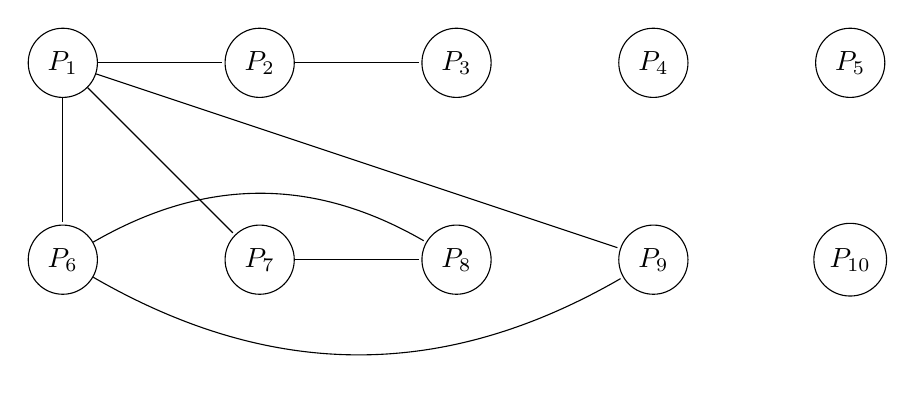
\begin{tikzpicture}[-,>=stealth',shorten >=1pt,auto,node distance=2.5cm,
		scale = 1,transform shape]
		
		\node[state] (p1) {$P_{1}$};
		\node[state] (p2) [right of=p1] {$P_{2}$};
		\node[state] (p3) [right  of=p2] {$P_{3}$};
		\node[state] (p4) [right of=p3] {$P_{4}$};
		\node[state] (p5) [right of=p4] {$P_{5}$};

		\node[state] (p6) [below  of=p1] {$P_{6}$};
		\node[state] (p7) [right of=p6] {$P_{7}$};
		\node[state] (p8) [right of=p7] {$P_{8}$};
		\node[state] (p9) [right of=p8] {$P_{9}$};
		\node[state] (p10) [right of=p9] {$P_{10}$};

		\path 
		(p1) edge          		 node{}(p2)
		(p1) edge          		 node{}(p6)
		(p1) edge          		 node{}(p7)
		(p1) edge          		 node{}(p9)
		(p2) edge          		 node{}(p3)
		(p6) edge[bend left]     node{}(p8)
		(p6) edge[bend right]    node{}(p9)
		(p7) edge          		 node{}(p8);
		\end{tikzpicture}
	\end{center}

	\begin{center}
		\begin{tabular}{c c c}
			 & Maximal Cliques & \\
			\hline \hline
			$\{P_1,P_2\}$ & $\{P_1, P_6, P_9\}$ & $\{P_1, P_7\}$ \\	
			$\{P_7,P_8\}$ & $\{P_6, P_8\}$ 		& $\{P_2, P_3\}$ \\
			$\{P_4\}$ 	  & $\{P_5\}$ 			& $\{P_{10}\}$
		\end{tabular}
	\end{center}
	\item \textbf{Determine the canonical heuristic $h^{\pazocal{C}}$
	and simplify it as much as possible}
	\begin{multicols}{3}
		\begin{tabular}{c c}
			$ i $		& $h^{P_i}$\\
			\hline\hline
			1 & 1 \\
			2 & 5 \\
			3 & 4 \\
			4 & 13\\
			5 & 0 \\
			6 & 1 \\
			7 & 1 \\
			8 & 1 \\
			9 & 0 \\
			10& 1 \\
		\end{tabular}

		\begin{tabular}{l | c}
			\multicolumn{2}{c}{Cliques heuristics} \\
			\hline \hline
			Clique & $h^{\pazocal{C}}$\\
			\hline
			$\{P_1,P_2\}$ 		& 6 \\
			$\{P_1, P_6, P_9\}$ & 2 \\
			$\{P_1, P_7\}$ 		& 2 \\
			$\{P_7,P_8\}$ 		& 2 \\
			$\{P_6, P_8\}$ 		& 2 \\
			$\{P_2, P_3\}$ 		& 9 \\
			$\{P_4\}$ 	  		& 13\\
			$\{P_5\}$ 			& 0 \\
			$\{P_{10}\}$		& 1
		\end{tabular}

		\[ h^{\pazocal{C}}=13\]
	\end{multicols}
	\item \textbf{Which patterns in $\pazocal{C}$ can be omitted and why?}
	\item \textbf{What would the canonical heuristic look like if we omitted
	those patterns before even constructing the compatibility graph}
\end{enumerate}

%%%%%%%%%%%%%%%%%%%%%  Ejercicio 2 %%%%%%%%%%%%%%%%%%%%%%%%%
\section*{Exercise 9.2 - Orthogonality and pairwise orthogonality}

\end{document}